% Beamer Presentation
% LaTeX Template
% Version 1.0 (10/11/12)
%
% This template has been downloaded from:
% http://www.LaTeXTemplates.com
%
% License:
% CC BY-NC-SA 3.0 (http://creativecommons.org/licenses/by-nc-sa/3.0/)
%
% Modified into a Beamer template for Northwestern University,
% by Daniel Lynch, 2019.
%
%%%%%%%%%%%%%%%%%%%%%%%%%%%%%%%%%%%%%%%%%

%----------------------------------------------------------------------------------------
%	PACKAGES AND THEMES
%----------------------------------------------------------------------------------------

\documentclass[aspectratio=169,9pt,xcolor=dvipsnames]{beamer}

\mode<presentation> {

% The Beamer class comes with a number of default slide themes
% which change the colors and layouts of slides. Below this is a list
% of all the themes, uncomment each in turn to see what they look like.

%\usetheme{default}
%\usetheme{AnnArbor}
%\usetheme{Antibes}
%\usetheme{Bergen}
\usetheme[hideothersubsections]{Berkeley}
%\usetheme{Berlin}
%\usetheme{Boadilla}
%\usetheme{CambridgeUS}
%\usetheme{Copenhagen}
%\usetheme{Darmstadt}
%\usetheme{Dresden}
%\usetheme{Frankfurt}
%\usetheme{Goettingen}
%\usetheme{Hannover}
%\usetheme{Ilmenau}
%\usetheme{JuanLesPins}
%\usetheme{Luebeck}
%\usetheme{Madrid}
%\usetheme{Malmoe}
%\usetheme{Marburg}
%\usetheme{Montpellier}
%\usetheme{PaloAlto}
%\usetheme{Pittsburgh}
%\usetheme{Rochester}
%\usetheme{Singapore}
%\usetheme{Szeged}
%\usetheme{Warsaw}

% As well as themes, the Beamer class has a number of color themes
% for any slide theme. Uncomment each of these in turn to see how it
% changes the colors of your current slide theme.

%\usecolortheme{albatross}
%\usecolortheme{beaver}
%\usecolortheme{beetle}
%\usecolortheme{crane}
%\usecolortheme{dolphin}
%\usecolortheme{dove}
%\usecolortheme{fly}
%\usecolortheme{lily}
%\usecolortheme{orchid}
%\usecolortheme{rose}
%\usecolortheme{seagull}
\usecolortheme{seahorse}
%\usecolortheme{whale}
%\usecolortheme{wolverine}

% Define NU color scheme:
% https://www.mccormick.northwestern.edu/marketing/logos-and-branding/color-usage-guidelines.html
\definecolor{NUpurple}{RGB}{078,042,132} % Northwestern Purple PMS 268, 0x4e2a84
\definecolor{purple60}{RGB}{131,110,170} % Purple 60, 0x836eaa
\definecolor{purple30}{RGB}{182,172,209} % Purple 30, 0xb6acd1
\definecolor{purple10}{RGB}{228,224,238} % Purple 10, 0xe4e0ee
\definecolor{purple120}{RGB}{064,031,104} % Purple 120, 0x401f68
\definecolor{black80}{HTML}{342F2E}     % Rich Black 80
\definecolor{black80}{HTML}{716C6B}     % Rich Black 50
\definecolor{black80}{HTML}{BBB8B8}     % Rich Black 20
\definecolor{black80}{HTML}{D8D6D6}     % Rich Black 10

\setbeamercolor{palette primary}{bg=NUpurple,fg=white}
\setbeamercolor{palette secondary}{bg=NUpurple,fg=white}
\setbeamercolor{palette tertiary}{bg=NUpurple,fg=white}
\setbeamercolor{palette quaternary}{bg=NUpurple,fg=white}
\setbeamercolor{structure}{fg=NUpurple} % itemize, enumerate, etc
\setbeamercolor{section in toc}{fg=NUpurple} % TOC sections

%\setbeamertemplate{footline} % To remove the footer line in all slides uncomment this line
\setbeamertemplate{footline}[page number] % To replace the footer line in all slides with a simple slide count uncomment this line

\setbeamertemplate{navigation symbols}{} % To remove the navigation symbols from the bottom of all slides uncomment this line
}

\usepackage{amsmath}
\usepackage{graphicx} % Allows including images
\usepackage{multimedia}
\usepackage{media9}
\usepackage{booktabs} % Allows the use of \toprule, \midrule and \bottomrule in tables
%\usepackage[orientation=landscape,size=custom,width=16,height=9,scale=0.5,debug]{beamerposter}
\usepackage{caption}
\captionsetup[figure]{labelformat=empty}% redefines the caption setup of the figures environment in the beamer class.
\usepackage{textpos}
\usepackage{tikz}
\usepackage{pgfpages}
\usepackage{listings}

%----------------------------------------------------------------------------------------
% CUSTOM MACROS
%----------------------------------------------------------------------------------------
\newcommand{\etal}{et al. }
\newcommand{\ie}{i.e., }
\newcommand{\eg}{e.g., }

%----------------------------------------------------------------------------------------
%	TITLE PAGE
%----------------------------------------------------------------------------------------

\title[Intro]{LLMs for Citation Management} % The short title appears at the bottom of every slide, the full title is only on the title page

\author[Aerith Netzer]{Aerith Netzer} % Your name
\institute[NU] % Your institution as it will appear on the bottom of every slide, may be shorthand to save space
{
Digital Publishing and Repository Librarian \\ % Your institution for the title page
\medskip
Northwestern University Libraries \\ % Your institution for the title page
\medskip
\textit{aerith.netzer@northwestern.edu} % Your email address
}
\date{\today} % Date, can be changed to a custom date

\begin{document}

\begin{frame}
\titlepage % Print the title page as the first slide
%\maketitle
%\vspace{-2.5cm}
%\includegraphics[width=\textwidth]{titleslide.eps}
\end{frame}

\addtobeamertemplate{frametitle}{}{
\begin{textblock*}{100mm}(.72\textwidth,-0.72cm)
\vspace{-0.1cm}

\includegraphics[width=4cm]{lockup-horizontal-short-white-rgb.eps}
\end{textblock*}}

%----------------------------------------------------------------------------------------
%	PRESENTATION SLIDES
%----------------------------------------------------------------------------------------

\begin{frame}
\frametitle{FOSS}
\begin{block}{This Presentation and its code is available on GitHub}
    \begin{itemize}
        \item \url{https://www.GitHub.com/aerithnetzer/OpenAI_Presentation}

\end{block}
\end{frame}

%------------------------------------------------

\section{Background} % Sections can be created in order to organize your presentation into discrete blocks, all sections and subsections are automatically printed in the table of contents as an overview of the talk
%------------------------------------------------
\subsection{Current State}
\begin{frame}
    \frametitle{Current State}
    \begin{center}
        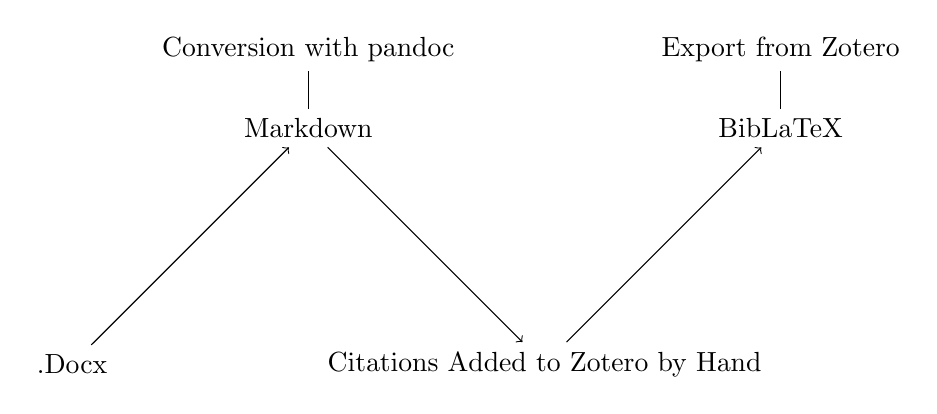
\begin{tikzpicture}
            \node (docx) at (0,0) {.Docx};
            \node (markdown) at (3,3) {Markdown};
            \node (zotero) at (6,0) {Citations Added to Zotero by Hand};
            \node (biblatex) at (9,3) {BibLaTeX};
            \node (pandoc) at (3,4) {Conversion with pandoc};
            \node (export) at (9,4) {Export from Zotero};
            
            \draw[->] (docx) -- (markdown);
            \draw[->] (markdown) -- (zotero);
            \draw[->] (zotero) -- (biblatex);
            \draw[-] (markdown) -- (pandoc);
            \draw[-] (biblatex) -- (export);
        \end{tikzpicture}
    \end{center}
        \begin{block}{The Current State Is Not Scalable}
            \begin{itemize}
                \item The current process is time-consuming
                \item The current process is error-prone
                \item The current process is not scalable
            \end{itemize}
        \end{block}
        
\end{frame}

\subsection{Problem \& Solution}
\begin{frame}[t]
    \frametitle{Solving Problems That We Created}
    \begin{block}{The problem of plaintext citations}
        \begin{itemize}
            \item Plaintext citations are not machine-readable
            \item Many different citation styles cause confusion
            \item Citations are often not linked to the cited work
        \end{itemize}
    \end{block}
    \begin{block}{The Suboptimal Solution: OpenAI GPT-3.5}
        \begin{itemize}
            \item Parse citations from article submission
            \item Create a .txt file with the citations in plaintext
            \item Call the OpenAI API to generate a biblatex file
        \end{itemize}
    \end{block}
\begin{block}{The Optimal Solution: Bib\LaTeX\ Evangelising}
    \begin{itemize}
        \item Create resources that help create .bib files
        \item Communicate the importance of Bib\LaTeX\ to researchers
        \item Create a .tex file with the citations in BibLaTeX
    \end{itemize}


\end{block}
\centering
\end{frame}
%------------------------------------------------

%----------------------------------------------------------------------------------------

\end{document} 
